% !TeX spellcheck = ru_RU
% !TEX root = vkr.tex

\section{Обучение классификатора отбора листьев}
\label{sec:classifier_chapter}

\subsection{Постановка задачи}
\label{sec:classifier_task}

После сегментации (раздел~\ref{sec:auto_mode}) получается набор
масок-кандидатов всех объектов на изображении: и корректные одиночные
листья, пригодные для измерений, и брак~--- повреждённые, перекрывающиеся,
нелистовые артефакты. Для отбора пригодных листьев обучается отдельный
классификатор. Вход модели~--- канонический RGB-фрагмент
(раздел~\ref{sec:pipeline}). Выход~--- метка одного из трёх классов:

\begin{itemize}
    \item \texttt{good\_leaf}~--- корректный одиночный лист, пригодный для
          морфометрических измерений;
    \item \texttt{bad\_leaf}~--- лист с дефектами (перекрытия с другими
          объектами, неполная форма, рваные края);
    \item \texttt{non\_leaf}~--- объект нелистовой природы (фон, тень,
          артефакт сегментации).
\end{itemize}

Стоимость ошибок классификатора несимметрична: пропущенный лист
безвозвратно теряется, тогда как ложно положительный фрагмент попадает в
итоговую таблицу измерений и удаляется вручную. Поэтому в качестве рабочей
точки фиксируется уровень recall $\geq 0{,}95$ на позитивном классе
\texttt{good\_leaf}~--- гарантия, что не более $\sim 5\,\%$ корректных
листьев теряется на этапе фильтрации. Соответствующая precision при этом
recall используется как основная метрика качества по всей главе.

\subsection{Архитектура классификатора}
\label{sec:classifier}

Малый объём ручной разметки ($\sim 100\!-\!600$ позитивных примеров на тип
листа, см.\ табл.~\ref{tab:clf_balance}) исключает дообучение свёрточной сети
целиком~--- риск переобучения слишком высок. Поэтому классификатор реализован
как двухэтапная модель: замороженный экстрактор признаков на основе свёрточной
сети, предобученной на ImageNet, и градиентный бустинг XGBoost, обучаемый на
этих признаках (рис.~\ref{fig:classifier_pipeline}).

\begin{figure}[H]
    \centering
    \begin{tikzpicture}[
        font=\scriptsize,
        box/.style={rectangle, draw, rounded corners=2pt,
                    minimum height=1.5cm, align=center, fill=gray!4,
                    inner sep=4pt},
        arr/.style={->, >=Stealth, thick},
        node distance=0.45cm,
    ]
    \node[inner sep=0pt] (img)
        {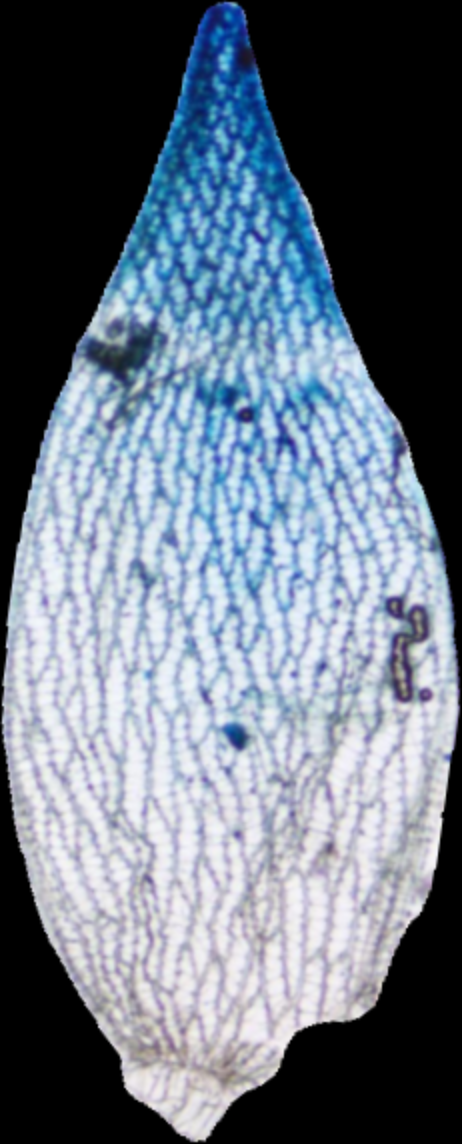
\includegraphics[height=1.9cm]{figures/121_170_0035_leaf_crop_0002.png}};
    \node[inner sep=0pt, right=of img] (letter)
        {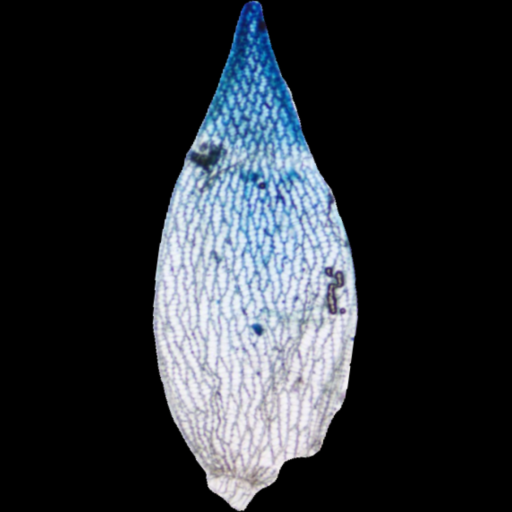
\includegraphics[height=1.9cm]{figures/121_170_0035_leaf_crop_0002_letterbox.png}};
    \node[box, right=of letter, minimum width=2.6cm, fill=blue!8] (mnet)
        {MobileNetV3-Small\\(заморожена)};
    \node[box, right=of mnet, minimum width=1.7cm] (feat)
        {576\\признаков};
    \node[box, right=of feat, minimum width=2.4cm, fill=orange!10] (xgb)
        {XGBoost\\300 деревьев};
    \node[box, right=of xgb, minimum width=1.9cm] (out)
        {\texttt{good\_leaf}\\\texttt{bad\_leaf}\\\texttt{non\_leaf}};
    \foreach \a/\b in {img/letter, letter/mnet, mnet/feat, feat/xgb, xgb/out}
        \draw[arr] (\a.east) -- (\b.west);
    \end{tikzpicture}
    \caption{Конвейер классификатора отбора масок}
    \label{fig:classifier_pipeline}
\end{figure}

\subsubsection*{Извлечение признаков}

Используется MobileNetV3-Small из \texttt{torchvision}, предобученная на
ImageNet. Финальный классификационный слой заменяется на \texttt{Identity}
(сеть возвращает 576-мерный эмбеддинг вместо 1000 ImageNet-логитов), все
параметры заморожены. Каждый фрагмент
вписывается в квадрат $512 \times 512$ пикселей с сохранением пропорций, нормализуется по статистикам ImageNet
и пропускается через сеть; на выходе~--- вектор $576$ признаков.

\subsubsection*{Параметры XGBoost}

XGBoost (\texttt{XGBClassifier}, \texttt{multi:softprob}) с гиперпараметрами:
$300$ деревьев, максимальная глубина $6$, темп обучения $0{,}1$,
\texttt{subsample}$\,= 0{,}8$, \texttt{colsample\_bytree}$\,= 0{,}8$,
\texttt{tree\_method}$\,=$ \texttt{"hist"}. Веса классов компенсируют
дисбаланс ($\sim 100\!-\!600$ позитивных против $1500$ \texttt{bad\_leaf} и
$\sim 1000$ \texttt{non\_leaf}) и задаются формулой:
\begin{equation}
    w_c = \frac{N_{\text{total}}}{n_{\text{classes}} \cdot N_c},
    \label{eq:class_weights}
\end{equation}
где $N_c$~--- число примеров класса~$c$, $N_{\text{total}}$~--- общий размер
обучающей выборки. Обоснование выбора численных значений приведено в
разделе~\ref{sec:classifier_justification}.

\subsection{Сбор обучающей выборки}
\label{sec:classifier_dataset}

Размеченная выборка собрана автором работы с использованием интерактивного
режима приложения (раздел~\ref{sec:interactive}): на каждом исходном снимке
запускалась автосегментация, полученные кандидаты вручную распределялись по
трём классам.

Морфология листьев у разных групп \textit{Sphagnum} существенно различается, поэтому
позитивный класс \texttt{good\_leaf\_<type>} собран отдельно для каждого из
трёх типов, а отказные классы \texttt{bad\_leaf} (повреждённые или перекрытые
листья) и \texttt{non\_leaf} (артефакты сегментации, фон, тени)~--- общие для
всех типов и не требуют повторной разметки. Полный датасет
опубликован: \url{https://cloud.mail.ru/public/jvB9/ReNV4TrpS}.

\begin{table}[H]
\centering
\caption{Распределение классов в обучающей выборке (по типам листа)}
\label{tab:clf_balance}
\small
\begin{tabular}{lcccc}
\hline
\textbf{Тип листа} & \texttt{good\_leaf} & \texttt{bad\_leaf} & \texttt{non\_leaf} & \textbf{Доля \texttt{good}} \\
\hline
\texttt{branch}        & 566  & 1500 & 994  & $18{,}5\,\%$ \\
\texttt{capillifolium} & 121  & 1500 & 994  & $4{,}6\,\%$  \\
\texttt{girgensohnii}  & 309  & 1500 & 994  & $11{,}0\,\%$ \\
\hline
\end{tabular}
\end{table}

\subsubsection*{Аугментация}

Каждый фрагмент размножается в шесть детерминированных вариантов: горизонтальное
отражение (два состояния), перемноженное на три цветовые трансформации~---
оригинал, осветление и затемнение по яркости, контрасту и насыщенности.
Вертикальное отражение нарушило бы инвариант ``апекс сверху'' и не
используется. Признаки MobileNetV3 вычисляются для каждого варианта один раз
и кэшируются.

\subsection{Результаты}
\label{sec:classifier_results}

Качество оценивается $5$-кратной стратифицированной кросс-валидацией; на
обучающих разбиениях применяется шестикратная аугментация, тестовое
разбиение проходит без аугментации. По накопленным предсказаниям пяти
разбиений в бинарной задаче \texttt{good\_leaf} против объединения
\texttt{bad\_leaf} и \texttt{non\_leaf} для каждого типа листа найден
минимальный порог $p_{\text{good}}$, при котором recall $\geq 0{,}95$
(рис.~\ref{fig:clf_pr_curve}).

\begin{figure}[H]
    \centering
    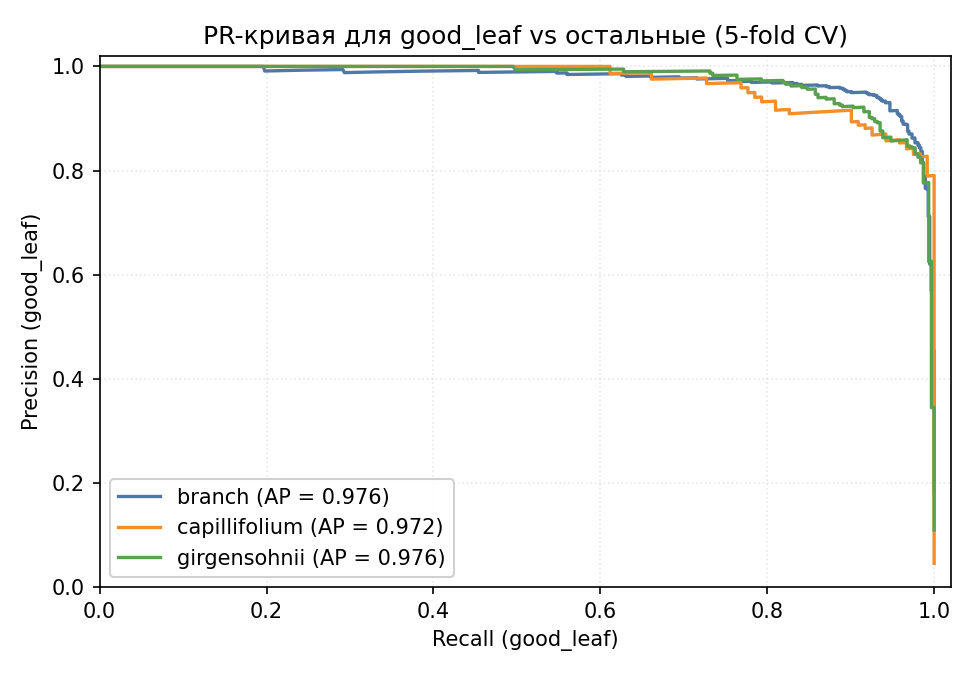
\includegraphics[width=0.6\linewidth]{figures/classifier_pr_curve.png}
    \caption{PR-кривая классификатора для бинарной задачи
    \texttt{good\_leaf} против остальных классов (5-кратная
    кросс-валидация)}
    \label{fig:clf_pr_curve}
\end{figure}

\begin{table}[H]
\centering
\caption{Метрики классификатора на рабочей точке recall $\geq 0{,}95$
(5-кратная кросс-валидация)}
\label{tab:clf_metrics}
\small
\begin{tabular}{lccccc}
\hline
\textbf{Тип листа} & $\boldsymbol{p_{\text{good}}}$ &
\textbf{Precision} & \textbf{Recall} & \textbf{F1} & \textbf{AP} \\
\hline
\texttt{branch}        & $0{,}22$ & $0{,}921 \pm 0{,}027$ & $0{,}95$ & $0{,}935$ & $0{,}977 \pm 0{,}009$ \\
\texttt{capillifolium} & $0{,}24$ & $0{,}884 \pm 0{,}050$ & $0{,}95$ & $0{,}916$ & $0{,}972 \pm 0{,}014$ \\
\texttt{girgensohnii}  & $0{,}12$ & $0{,}882 \pm 0{,}049$ & $0{,}95$ & $0{,}915$ & $0{,}978 \pm 0{,}009$ \\
\hline
\end{tabular}
\end{table}

Precision и AP даны как среднее по 5 фолдам $\pm$ стандартное отклонение
между фолдами. На всех трёх типах достигнут целевой recall при precision
$0{,}88\!-\!0{,}92$. Площадь под PR-кривой $> 0{,}97$ для всех типов
означает, что модель хорошо разделяет позитивный класс почти на всём
диапазоне порогов. Минимальная precision на \texttt{capillifolium} и
\texttt{girgensohnii} связана с меньшим объёмом размеченных позитивных
примеров ($121$ и $309$ против $566$ для \texttt{branch}).

Разброс по фолдам ($\pm 2{,}7$\,п.п.\ на \texttt{branch}, $\pm 5$\,п.п.\
на \texttt{capillifolium} и \texttt{girgensohnii}) при усреднении по 5
разбиениям даёт стандартную ошибку среднего
$\sigma_{\text{CV}} \approx 1\!-\!2$\,п.п.~--- этим определяется уровень
шума при сравнении архитектурных вариантов в
разделе~\ref{sec:classifier_justification}.

\subsection{Сравнение с альтернативными архитектурами}
\label{sec:classifier_justification}

Каждое архитектурное решение проверено отдельным экспериментом по тому же
протоколу 5-кратной кросс-валидации, что и в табл.~\ref{tab:clf_metrics};
метрика~--- precision при recall $= 0{,}95$ на классе \texttt{good\_leaf}. Прикладные ограничения, принимаемые во внимание при
выборе архитектуры: вычисления на CPU рабочей станции лаборатории, малый
объём ручной разметки ($\sim 100\!-\!600$ позитивных примеров на тип листа),
повторное обучение силами лаборатории при добавлении нового типа.

\subsubsection*{Выбор сети-экстрактора признаков}

Сравнивались восемь замороженных экстракторов признаков с фиксированным
итоговым классификатором XGBoost (табл.~\ref{tab:clf_backbones}).

\begin{table}[H]
\centering
\caption{Precision при recall $= 0{,}95$ для разных экстракторов признаков}
\label{tab:clf_backbones}
\scriptsize
\begin{tabular}{lcccrr}
\hline
\textbf{Экстрактор} & \textbf{branch} & \textbf{capilli.} & \textbf{girgens.} &
\textbf{CPU,\,мс} & \textbf{Вес,\,МБ} \\
\hline
\textbf{MobileNetV3-Small (выбран)} & $\mathbf{0{,}913 \pm 0{,}049}$ & $\mathbf{0{,}896 \pm 0{,}039}$ & $0{,}889 \pm 0{,}030$ & $\mathbf{6}$ & $\mathbf{9{,}7}$ \\
EfficientNet-B0    & $0{,}901 \pm 0{,}038$ & $0{,}826 \pm 0{,}048$ & $0{,}904 \pm 0{,}027$ & $13$  & $20{,}5$ \\
DINOv2-small       & $0{,}882 \pm 0{,}035$ & $\mathbf{0{,}896 \pm 0{,}109}$ & $\mathbf{0{,}911 \pm 0{,}029}$ & $192$ & $84{,}2$ \\
MobileNetV3-Large  & $0{,}874 \pm 0{,}006$ & $0{,}841 \pm 0{,}062$ & $0{,}877 \pm 0{,}044$ & $16$  & $21{,}0$ \\
ResNet-50          & $0{,}896 \pm 0{,}015$ & $0{,}875 \pm 0{,}108$ & $0{,}889 \pm 0{,}013$ & $25$  & $97{,}8$ \\
ConvNeXt-Tiny      & $0{,}879 \pm 0{,}044$ & $0{,}857 \pm 0{,}034$ & $0{,}898 \pm 0{,}020$ & $25$  & $109{,}1$ \\
ResNet-18          & $0{,}872 \pm 0{,}027$ & $0{,}740 \pm 0{,}142$ & $0{,}886 \pm 0{,}046$ & $11$  & $44{,}7$ \\
MobileSAM-encoder  & $0{,}772 \pm 0{,}069$ & $0{,}686 \pm 0{,}081$ & $0{,}801 \pm 0{,}036$ & $347$ & $38{,}8$ \\
\hline
\end{tabular}
\end{table}

MobileNetV3-Small лидирует на \texttt{branch} (самой крупной выборке) и
\texttt{capillifolium}, на \texttt{girgensohnii} уступает DINOv2-small на
$2{,}2$\,п.п.~--- в пределах CV-шума $\sigma_{\text{CV}}$. DINOv2
проигрывает в $32$ раза по скорости и в $8{,}7$ раза по объёму весов~---
неприемлемо для рабочей станции без GPU. Кодировщик MobileSAM
(переиспользование весов сегментатора) даёт просадку
$8{,}8\!-\!21{,}0$\,п.п.\ при $58$-кратном замедлении~--- разрыв
кратно превышает шум, эта замена однозначно отвергается.

\subsubsection*{Сравнение глубоких и ручных признаков}

Морфометрическая базовая модель на $84$ ручных признаках (форма и площадь,
профиль ширины, эллиптические Фурье-дескрипторы, моменты Ху, симметрия,
кривизна у апекса) с тем же XGBoost сравнена с признаками MobileNet
(табл.~\ref{tab:clf_features}).

\begin{table}[H]
\centering
\caption{Precision при recall $= 0{,}95$: глубокие и ручные признаки}
\label{tab:clf_features}
\small
\begin{tabular}{lccc}
\hline
\textbf{Признаки} & \textbf{branch} & \textbf{capilli.} & \textbf{girgens.} \\
\hline
\textbf{MobileNetV3-Small (576-d, выбран)} & $\mathbf{0{,}913 \pm 0{,}049}$ & $\mathbf{0{,}896 \pm 0{,}039}$ & $\mathbf{0{,}889 \pm 0{,}030}$ \\
$84$ ручных & $0{,}793 \pm 0{,}074$ & $0{,}577 \pm 0{,}159$ & $0{,}616 \pm 0{,}052$ \\
\hline
\end{tabular}
\end{table}

Разрыв $12{,}0\!-\!31{,}9$\,п.п.\ означает, что контурная геометрия не
описывает текстурный сигнал, существенный для отбраковки повреждённых и
нелистовых объектов.

\subsubsection*{Выбор классификатора}

На зафиксированных признаках MobileNet сравнивались шесть альтернатив XGBoost
(табл.~\ref{tab:clf_models}).

\begin{table}[H]
\centering
\caption{Precision при recall $= 0{,}95$ для разных классификаторов поверх
признаков MobileNetV3-Small}
\label{tab:clf_models}
\small
\begin{tabular}{lccc}
\hline
\textbf{Модель} & \textbf{branch} & \textbf{capilli.} & \textbf{girgens.} \\
\hline
\textbf{XGBoost (выбран)} & $\mathbf{0{,}921 \pm 0{,}027}$ & $0{,}884 \pm 0{,}050$ & $0{,}882 \pm 0{,}049$ \\
RBF-SVM       & $0{,}888 \pm 0{,}039$ & $0{,}906 \pm 0{,}052$ & $\mathbf{0{,}918 \pm 0{,}036}$ \\
MLP           & $0{,}892 \pm 0{,}037$ & $\mathbf{0{,}911 \pm 0{,}059}$ & $0{,}897 \pm 0{,}025$ \\
LogReg        & $0{,}860 \pm 0{,}050$ & $0{,}876 \pm 0{,}093$ & $0{,}845 \pm 0{,}039$ \\
RandomForest  & $0{,}862 \pm 0{,}035$ & $0{,}717 \pm 0{,}096$ & $0{,}873 \pm 0{,}049$ \\
LinearSVM     & $0{,}814 \pm 0{,}015$ & $0{,}822 \pm 0{,}064$ & $0{,}877 \pm 0{,}034$ \\
kNN           & $0{,}801 \pm 0{,}056$ & $0{,}749 \pm 0{,}092$ & $0{,}821 \pm 0{,}052$ \\
\hline
\end{tabular}
\end{table}

XGBoost~--- лидер на \texttt{branch} (самой крупной выборке); на
\texttt{capillifolium} и \texttt{girgensohnii} он уступает MLP и RBF-SVM
на $2{,}7\!-\!3{,}6$\,п.п.~--- порядка $1\!-\!2\,\sigma_{\text{CV}}$, на
грани шума и без устойчивого преимущества альтернатив. XGBoost оставлен
как лидер на самой крупной выборке плюс встроенная поддержка
\texttt{sample\_weight} для компенсации дисбаланса. Линейные модели
(LogReg, LinearSVM) и kNN отстают на $5\!-\!10$\,п.п.~--- разрыв
кратно превышает шум.

\subsubsection*{Параметры XGBoost}

Для проверки выбранных значений и оценки, нужна ли отдельная подстройка
под каждый тип листа, выполнен поиск по сетке (\texttt{n\_estimators}
$\in [50;\,1500]$, \texttt{max\_depth} $\in [2;\,12]$,
\texttt{learning\_rate} $\in [0{,}01;\,0{,}3]$, \texttt{subsample},
\texttt{colsample\_bytree} $\in [0{,}5;\,1{,}0]$): каждый параметр
перебирался независимо при остальных, зафиксированных на выбранных
значениях.

\begin{figure}[H]
\centering
\begin{tikzpicture}
\begin{axis}[
    width=0.85\linewidth, height=6.5cm,
    xlabel={Число деревьев $n_{\text{est}}$},
    ylabel={precision при recall $= 0{,}95$},
    xmin=0, xmax=1280,
    ymin=0.82, ymax=0.93,
    legend style={at={(0.98,0.04)}, anchor=south east, font=\footnotesize,
                  draw=gray!50, fill=white, fill opacity=0.85,
                  text opacity=1},
    legend cell align={left},
    grid=major, grid style={dashed,gray!25},
    tick label style={font=\footnotesize},
    label style={font=\footnotesize},
    mark size=1.4pt,
]
\addplot[mark=*, color=blue!70!black, thick] coordinates {
    (50, 0.8911) (100, 0.8997) (150, 0.9139) (200, 0.9193)
    (300, 0.9208) (500, 0.9163) (800, 0.9161) (1200, 0.9147)
};
\addlegendentry{\texttt{branch}}
\addplot[mark=square*, color=red!70!black, thick] coordinates {
    (50, 0.8259) (100, 0.8574) (150, 0.8757) (200, 0.8761)
    (300, 0.8838) (500, 0.8969) (800, 0.8975) (1200, 0.8975)
};
\addlegendentry{\texttt{capillifolium}}
\addplot[mark=triangle*, color=green!50!black, thick] coordinates {
    (50, 0.8659) (100, 0.8665) (150, 0.8717) (200, 0.8751)
    (300, 0.8816) (500, 0.8841) (800, 0.8841) (1200, 0.8860)
};
\addlegendentry{\texttt{girgensohnii}}
\draw[dashed, gray!70, thick]
    (axis cs:300,0.82) -- (axis cs:300,0.93);
\node[gray!80, font=\footnotesize, anchor=south]
    at (axis cs:300,0.82) {\,300};
\end{axis}
\end{tikzpicture}
\caption{Зависимость precision (при recall $= 0{,}95$) от числа деревьев
XGBoost при остальных параметрах, фиксированных на выбранных значениях.
Пунктир~--- выбранное $n_{\text{est}} = 300$.}
\label{fig:clf_xgb_curve}
\end{figure}

На \texttt{branch} (самой крупной выборке) выбранные значения уже стоят
в максимуме сетки по всем пяти параметрам~--- одиночное изменение любого
из них только ухудшает precision. На меньших выборках
\texttt{capillifolium} и \texttt{girgensohnii} лучший прирост от
изменения одного параметра не превышает $2$\,п.п., что не выходит за
шум $\sigma_{\text{CV}}$. Лучшие значения по разным типам листа взаимно
противоречат (например, \texttt{max\_depth}: $6$ / $4$ / $5$;
\texttt{subsample}: $0{,}8$ / $0{,}7$ / $1{,}0$)~--- характерное
проявление переобучения на конкретные разбиения, а не сигнал о наличии
предпочтительной конфигурации под отдельный тип. Поэтому единая
конфигурация $(\texttt{n\_estimators} = 300$, $\texttt{max\_depth} = 6$,
$\texttt{learning\_rate} = 0{,}1$, $\texttt{subsample} = 0{,}8$,
$\texttt{colsample\_bytree} = 0{,}8)$ оставлена для всех трёх моделей.

\subsubsection*{Число классов}

Бинарная постановка (\texttt{good} против объединения \texttt{bad} и
\texttt{non}) проверена на той же выборке и том же XGBoost
(табл.~\ref{tab:clf_classes}).

\begin{table}[H]
\centering
\caption{Precision при recall $= 0{,}95$: трёхклассовая и бинарная постановка}
\label{tab:clf_classes}
\small
\begin{tabular}{lccc}
\hline
\textbf{Постановка} & \textbf{branch} & \textbf{capilli.} & \textbf{girgens.} \\
\hline
\textbf{3 класса (выбрана)} & $\mathbf{0{,}921 \pm 0{,}027}$ & $\mathbf{0{,}884 \pm 0{,}050}$ & $0{,}882 \pm 0{,}049$ \\
2 класса (\texttt{good} против остального) & $0{,}895 \pm 0{,}042$ & $0{,}839 \pm 0{,}051$ & $\mathbf{0{,}896 \pm 0{,}044}$ \\
\hline
\end{tabular}
\end{table}

3-классовая постановка выигрывает на \texttt{branch} ($+2{,}6$\,п.п.) и
\texttt{capillifolium} ($+4{,}5$\,п.п., $\sim 2\sigma_{\text{CV}}$), уступает
на \texttt{girgensohnii} ($-1{,}5$\,п.п., в пределах $\sigma_{\text{CV}}$).
На самом малом позитивном классе (\texttt{capillifolium}, $121$ образец)
разрыв максимальный~--- различение типов отказа даёт дополнительный
обучающий сигнал, особенно ценный при малом числе положительных примеров.

\subsubsection*{Итог раздела}

Главный ограничитель качества классификатора~--- объём и качество
размеченной выборки (\texttt{capillifolium}~--- $121$ позитивный пример,
\texttt{girgensohnii}~--- $309$, табл.~\ref{tab:clf_balance}), а не
архитектурные решения: расширение и уточнение разметки сдвинут рабочую
точку существеннее любой замены сети-экстрактора, классификатора или
подстройки гиперпараметров.
